% Options for packages loaded elsewhere
\PassOptionsToPackage{unicode}{hyperref}
\PassOptionsToPackage{hyphens}{url}
\PassOptionsToPackage{dvipsnames,svgnames,x11names}{xcolor}
%
\documentclass[
  letterpaper,
  DIV=11,
  numbers=noendperiod]{scrartcl}

\usepackage{amsmath,amssymb}
\usepackage{iftex}
\ifPDFTeX
  \usepackage[T1]{fontenc}
  \usepackage[utf8]{inputenc}
  \usepackage{textcomp} % provide euro and other symbols
\else % if luatex or xetex
  \usepackage{unicode-math}
  \defaultfontfeatures{Scale=MatchLowercase}
  \defaultfontfeatures[\rmfamily]{Ligatures=TeX,Scale=1}
\fi
\usepackage{lmodern}
\ifPDFTeX\else  
    % xetex/luatex font selection
\fi
% Use upquote if available, for straight quotes in verbatim environments
\IfFileExists{upquote.sty}{\usepackage{upquote}}{}
\IfFileExists{microtype.sty}{% use microtype if available
  \usepackage[]{microtype}
  \UseMicrotypeSet[protrusion]{basicmath} % disable protrusion for tt fonts
}{}
\makeatletter
\@ifundefined{KOMAClassName}{% if non-KOMA class
  \IfFileExists{parskip.sty}{%
    \usepackage{parskip}
  }{% else
    \setlength{\parindent}{0pt}
    \setlength{\parskip}{6pt plus 2pt minus 1pt}}
}{% if KOMA class
  \KOMAoptions{parskip=half}}
\makeatother
\usepackage{xcolor}
\setlength{\emergencystretch}{3em} % prevent overfull lines
\setcounter{secnumdepth}{-\maxdimen} % remove section numbering
% Make \paragraph and \subparagraph free-standing
\makeatletter
\ifx\paragraph\undefined\else
  \let\oldparagraph\paragraph
  \renewcommand{\paragraph}{
    \@ifstar
      \xxxParagraphStar
      \xxxParagraphNoStar
  }
  \newcommand{\xxxParagraphStar}[1]{\oldparagraph*{#1}\mbox{}}
  \newcommand{\xxxParagraphNoStar}[1]{\oldparagraph{#1}\mbox{}}
\fi
\ifx\subparagraph\undefined\else
  \let\oldsubparagraph\subparagraph
  \renewcommand{\subparagraph}{
    \@ifstar
      \xxxSubParagraphStar
      \xxxSubParagraphNoStar
  }
  \newcommand{\xxxSubParagraphStar}[1]{\oldsubparagraph*{#1}\mbox{}}
  \newcommand{\xxxSubParagraphNoStar}[1]{\oldsubparagraph{#1}\mbox{}}
\fi
\makeatother


\providecommand{\tightlist}{%
  \setlength{\itemsep}{0pt}\setlength{\parskip}{0pt}}\usepackage{longtable,booktabs,array}
\usepackage{calc} % for calculating minipage widths
% Correct order of tables after \paragraph or \subparagraph
\usepackage{etoolbox}
\makeatletter
\patchcmd\longtable{\par}{\if@noskipsec\mbox{}\fi\par}{}{}
\makeatother
% Allow footnotes in longtable head/foot
\IfFileExists{footnotehyper.sty}{\usepackage{footnotehyper}}{\usepackage{footnote}}
\makesavenoteenv{longtable}
\usepackage{graphicx}
\makeatletter
\newsavebox\pandoc@box
\newcommand*\pandocbounded[1]{% scales image to fit in text height/width
  \sbox\pandoc@box{#1}%
  \Gscale@div\@tempa{\textheight}{\dimexpr\ht\pandoc@box+\dp\pandoc@box\relax}%
  \Gscale@div\@tempb{\linewidth}{\wd\pandoc@box}%
  \ifdim\@tempb\p@<\@tempa\p@\let\@tempa\@tempb\fi% select the smaller of both
  \ifdim\@tempa\p@<\p@\scalebox{\@tempa}{\usebox\pandoc@box}%
  \else\usebox{\pandoc@box}%
  \fi%
}
% Set default figure placement to htbp
\def\fps@figure{htbp}
\makeatother

\usepackage{booktabs}
\usepackage{longtable}
\usepackage{array}
\usepackage{multirow}
\usepackage{wrapfig}
\usepackage{float}
\usepackage{colortbl}
\usepackage{pdflscape}
\usepackage{tabu}
\usepackage{threeparttable}
\usepackage{threeparttablex}
\usepackage[normalem]{ulem}
\usepackage{makecell}
\usepackage{xcolor}
\KOMAoption{captions}{tableheading}
\makeatletter
\@ifpackageloaded{caption}{}{\usepackage{caption}}
\AtBeginDocument{%
\ifdefined\contentsname
  \renewcommand*\contentsname{Table of contents}
\else
  \newcommand\contentsname{Table of contents}
\fi
\ifdefined\listfigurename
  \renewcommand*\listfigurename{List of Figures}
\else
  \newcommand\listfigurename{List of Figures}
\fi
\ifdefined\listtablename
  \renewcommand*\listtablename{List of Tables}
\else
  \newcommand\listtablename{List of Tables}
\fi
\ifdefined\figurename
  \renewcommand*\figurename{Figure}
\else
  \newcommand\figurename{Figure}
\fi
\ifdefined\tablename
  \renewcommand*\tablename{Table}
\else
  \newcommand\tablename{Table}
\fi
}
\@ifpackageloaded{float}{}{\usepackage{float}}
\floatstyle{ruled}
\@ifundefined{c@chapter}{\newfloat{codelisting}{h}{lop}}{\newfloat{codelisting}{h}{lop}[chapter]}
\floatname{codelisting}{Listing}
\newcommand*\listoflistings{\listof{codelisting}{List of Listings}}
\makeatother
\makeatletter
\makeatother
\makeatletter
\@ifpackageloaded{caption}{}{\usepackage{caption}}
\@ifpackageloaded{subcaption}{}{\usepackage{subcaption}}
\makeatother

\usepackage{bookmark}

\IfFileExists{xurl.sty}{\usepackage{xurl}}{} % add URL line breaks if available
\urlstyle{same} % disable monospaced font for URLs
\hypersetup{
  pdftitle={Music Mental Health Analysis},
  colorlinks=true,
  linkcolor={blue},
  filecolor={Maroon},
  citecolor={Blue},
  urlcolor={Blue},
  pdfcreator={LaTeX via pandoc}}


\title{Music Mental Health Analysis}
\usepackage{etoolbox}
\makeatletter
\providecommand{\subtitle}[1]{% add subtitle to \maketitle
  \apptocmd{\@title}{\par {\large #1 \par}}{}{}
}
\makeatother
\subtitle{Jordan Andrew}
\author{}
\date{}

\begin{document}
\maketitle


\begin{center}\rule{0.5\linewidth}{0.5pt}\end{center}

\section{Data}\label{data}

\subsection{Data Background}\label{data-background}

The data used in this analysis comes from the Music and Mental Health
(MxMH) Survey Results hosted on Kaggle. The dataset was collected
through an online Google Form that was distributed via social media and
public forums. It contains 736 respondents (rows) and includes variables
on demographic characteristics (such as age), music-listening habits
(hours per day, streaming platform, frequency of listening to certain
genres), and self-reported mental-health scores for anxiety, depression,
insomnia, and OCD (rated 0-10). The data is cross-sectional and
self-reported, meaning it is suitable for identifying
associations/correlations but not establishing causal effects.

\subsection{Data Cleaning}\label{data-cleaning}

Our data cleaning process began with an assessment of missing values
across all columns. This revealed 107 null entries in the BPM column and
a single null entry in the Age column. After looking further into the
BPM data collection, we discovered that it was meant to represent the
``Beats per minute of favorite genre.'' However, rows with the same
reported favorite genre displayed inconsistent BPM values, indicating
that participants did not interpret or answer the question reliably.
Combined with the large number of missing entries, this inconsistency
made the variable unsuitable for analysis, so we dropped the BPM column
entirely. The single row with a missing Age value was also removed to
maintain completeness for demographic modeling.

Next, we examined the dataset for implausible or erroneous entries.
During this process, we identified a respondent who reported being 89
years old and listening to music for 24 hours per day, and they were
doing so while working. Because this combination is not physically
possible and would exert undue influence on any model involving hours
per day, we removed this outlier from the dataset.

We then reviewed all variables designed to accept only binary ``Yes'' or
``No'' responses. Several of these columns contained values outside of
the allowed set, such as misspellings, alternative phrasing, or blank
entries. To maintain consistency in these binary predictors, we filtered
out any rows that did not provide valid ``Yes'' or ``No'' answers across
all such variables, resulting in the removal of nine additional rows.

After this, we checked the music effects variable and found seven cases
where respondents left this question blank. Because an empty string does
not constitute a valid category and this variable is used in later
modeling, we removed these seven rows as well.

For analyses involving streaming services, we examined the primary
streaming service column and identified two types of unusable entries:
blank responses and the explicit answer ``I do not use a streaming
service.'' Because our first research question specifically compares
listening patterns across streaming platforms, respondents without a
platform could not be meaningfully included in that analysis. Therefore,
for the dataset used in RQ1, we removed all rows with missing
streaming-service information as well as those who reported not using
any streaming service.

Finally, to prepare the binary outcome for our second research question,
we created a high depression variable that flags individuals with
elevated symptom levels. Because the average depression score in the
dataset was 4.82 and the median was 5, we designated respondents with a
score of 6 or higher as experiencing ``high depression.'' This threshold
represents a meaningful distinction between typical responses and
substantially elevated symptom reports, allowing us to model the
likelihood of more severe depression symptoms.

\section{Models}\label{models}

\subsection{Research Question 1: ``How does the number of hours spent
listening to music per day vary by depression status and primary
streaming
service?''}\label{research-question-1-how-does-the-number-of-hours-spent-listening-to-music-per-day-vary-by-depression-status-and-primary-streaming-service}

To investigate how the number of hours spent listening to music per day
varies based on depression symptoms and primary streaming service, we
fit a multiple linear regression model using hours per day as the
continuous response variable. Linear regression is appropriate for this
question because the goal is to estimate how the average listening
duration changes across different levels of depression and across
streaming platforms, while adjusting for potential confounders. We also
included an interaction term between depression and primary streaming
service, which tests whether the association between self-reported
depression symptoms and daily listening time differs by the platform a
respondent uses.

Beyond the primary predictors of depression and primary streaming
service, we included a set of covariates to reduce potential confounding
and isolate the effects of depression and steaming service on listening
time. These covariates were selected because they relate to both
music-listening behavior and mental-health-related characteristics
without making the model too busy. These covariates include age, while
working (whether the respondent listens while working), instrumentalist
(yes/no), composer (yes/no), exploratory (whether they tend to explore
new music), foreign languages (whether they tend to listen to music in
foreign languages), and three mental health related variables (anxiety,
insomnia, OCD, all self-reported on a scale of 0-10). We also included
two music-related behavioral factors, favorite genre and music effects,
to account for genre preferences and how individuals perceive music
impacts their emotions. Including these variables helps adjust for
individual differences in music engagement, mental-health comorbidity,
and daily listening contexts that could otherwise bias the estimated
relationships.

Our model, which follows the linear regression framework, relies on the
standard assumptions of linearity, independence of observations,
homoscedasticity, and normally distributed residuals. We also assumed
that there was no multicollinearity among predictors, and all of these
assumptions were assessed via diagnostic plots/tests.

\subsection{Research Question 2: ``Does the number of hours spent
listening to music each day increase the likelihood of reporting high
depression
symptoms?''}\label{research-question-2-does-the-number-of-hours-spent-listening-to-music-each-day-increase-the-likelihood-of-reporting-high-depression-symptoms}

For our second research question, which sought to determine if the
number of hours spent listening to music each day increases the
likelihood of reporting high depression symptoms, we fit a logistic
regression model with a binary outcome. Logistic regression is
appropriate because the response variable, high depression, classifies
respondents as either above or below a threshold level of self-reported
depressive symptoms, and the model estimates how the log-odds of being
in the high-depression category change with daily listening time.

Outside of our outcome variable of high depression and our primary
independent variable, daily hours spent listening to music, we also
included several covariates. Specifically, we adjusted for age,
indicators of music engagement (instrumentalist and composer),
co-occurring mental-health conditions (anxiety, insomnia, and OCD), and
two global music-use characteristics (favorite genre and music effects).
These variables may influence both how much an individual listens to
music and their underlying likelihood of experiencing elevated
depressive symptoms, thereby helping reduce confounding effects.

Logistic regression, and therefore our model, assumes independent
observations, linearity of continuous predictors on the log-odds scale,
and the absence of multicollinearity, all of which were checked via
plots and tests.

\section{Assessment and changes}\label{assessment-and-changes}

\subsection{Research Question 1}\label{research-question-1}

The first model we fit for RQ1 was a linear regression model that
regressed the raw outcome of hours of music listening per day on all
available predictors in the data set.

\pandocbounded{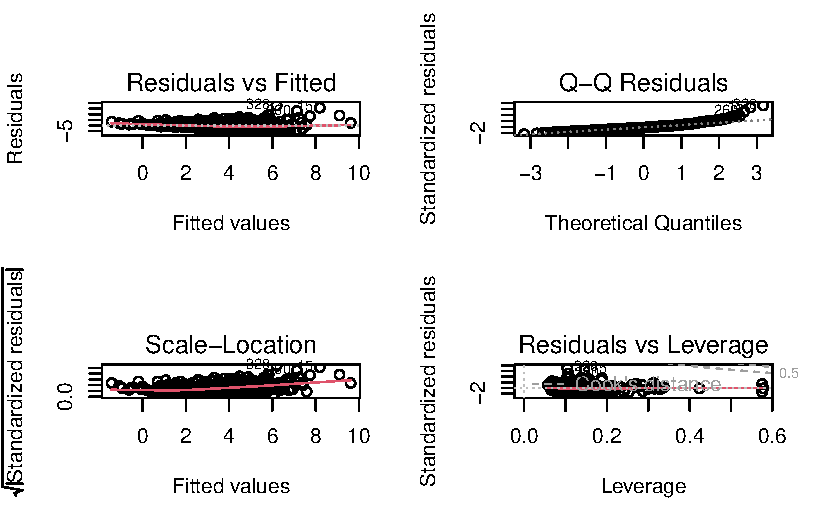
\includegraphics[keepaspectratio]{final_report_files/figure-pdf/unnamed-chunk-1-1.pdf}}

After fitting this initial model, we first examined the standard
diagnostic plots, as shown above: Residuals vs Fitted, Normal Q-Q,
Scale-Location, and Residuals vs.~Leverage. The Residuals vs Fitted plot
revealed a strong violation of homoscedasticity, with the points forming
a funnel-shape, and a small violation of linearity, where the red
smoothing line curved upward rather than remaining flat. The Normal Q--Q
plot showed noticeable departures from the 45 degree line, especially in
the upper tail, a clear strong violation of normality. The
Scale--Location plot further confirmed heteroscedasticity, with residual
spread increasing at higher fitted values. Finally, the Residuals
vs.~Leverage plot identified several influential observations with large
residuals and unusually high leverage, suggesting they were exerting
disproportionate influence on the fitted model.

After examining the diagnostic plots, we assessed multicollinearity
using GVIF values, which adjust for the degrees of freedom of
multi-level categorical variables. For most predictors, including age,
musician traits, mental-health indicators, and the genre-frequency
variables, the adjusted \(\text{GVIF}^{1/(2 \cdot \text{Df})}\) values
were all close to 1.1-1.3, indicating low multicollinearity and no
immediate concern for inflation of variance. The interaction term
between depression and primary streaming service also showed a modest
adjusted GVIF value of approximately 1.10, further supporting stability
in these estimates.

One exception was favorite genre, a 16-level categorical variable, which
produced a very large raw GVIF (≈ 2400). However, its adjusted value,
\(\text{GVIF}^{1/(2 \cdot \text{Df})} \approx 1.30\), fell well within
acceptable thresholds, since high raw GVIF numbers are expected for
factors with many degrees of freedom. No predictors exhibited adjusted
GVIF values approaching levels (≈ 2 or 3) that would indicate
problematic multicollinearity.

\pandocbounded{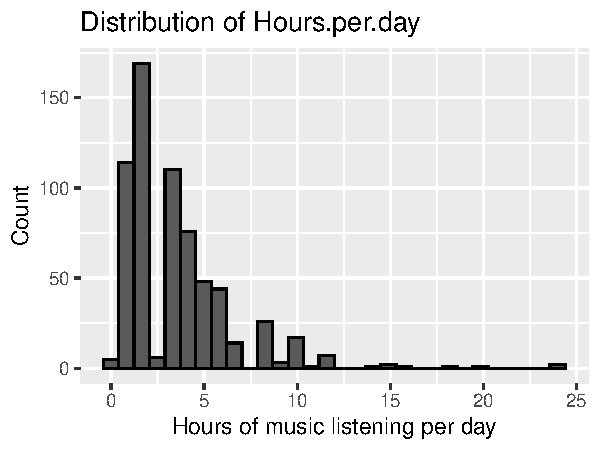
\includegraphics[keepaspectratio]{final_report_files/figure-pdf/p1-plot-1.pdf}}

Because the full model included many weakly justified predictors, we fit
a reduced model to improve parsimony and check whether the diagnostic
issues were caused by unnecessary complexity. We also inspected a
histogram of hours per day, pictured above, which was strongly
right-skewed, suggesting structural issues with the outcome itself. The
reduced model produced essentially the same adjusted R² (≈0.16) and
similar residual behavior, with persistent violations of linearity,
homoscedasticity, and normality, plus influential points. This showed
that removing predictors did not improve model fit and that the
underlying outcome distribution, not just model complexity, was driving
the diagnostic problems.

\pandocbounded{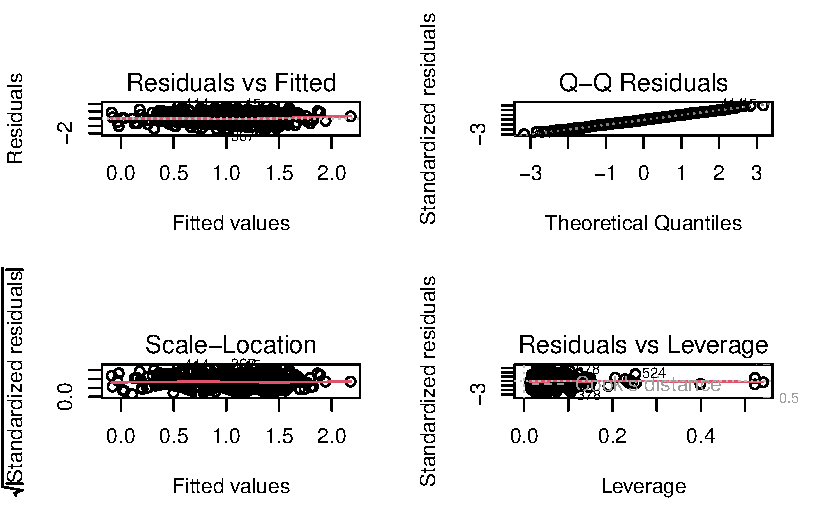
\includegraphics[keepaspectratio]{final_report_files/figure-pdf/unnamed-chunk-2-1.pdf}}

To address this we applied a log transformation to the outcome and
re--fit the model with \(\log(\text{Hours per day} + 0.1)\) as the
response. On the log scale, the Residuals vs fitted plot and Q--Q plot
showed substantially more symmetric and homoscedastic residuals (as
shown above) and the histogram of the transformed outcome indicated a
much more balanced distribution. These improvements suggested that the
log--transformed model better met the assumptions of linear regression.
We also used variance inflation factors (VIFs) to check for
multicollinearity among predictors and did not find strong evidence of a
violation.

\pandocbounded{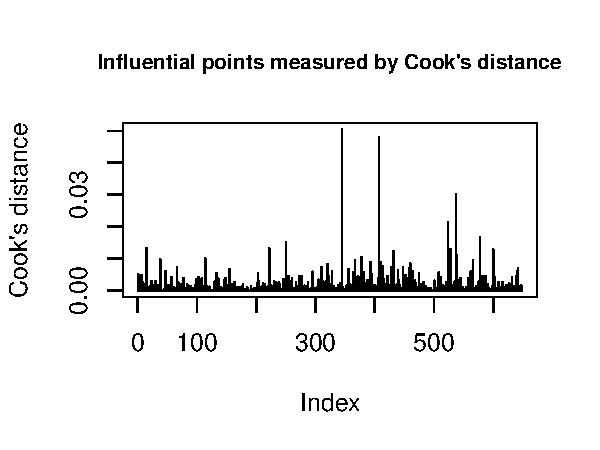
\includegraphics[keepaspectratio]{final_report_files/figure-pdf/unnamed-chunk-3-1.pdf}}

To evaluate influential observations, we computed Cook's distance for
the log-transformed RQ1 model and examined the corresponding plot. We
also inspected the residual and leverage diagnostic plots for outliers.
Combining these approaches, we identified three extreme points to
remove: two points were flagged as outliers in both the diagnostic plots
and Cook's distance, and one additional point appeared as an outlier
only in the diagnostic plots. After removing these three extreme points
, we refit the log-transformed model. The residuals are now more
symmetrically distributed (Min = -1.84, Max = 1.80, Median ≈ 0), and the
residual standard error decreased to 0.625, indicating improved model
fit.

Several predictors remain significant, including Depression, Primary
streaming service, While working, Instrumentalist, Composer, Insomnia,
and select favorite genres, with interactions between Depression and
streaming platform also holding. The adjusted \(R^2\) increased to
0.220, showing that the log transformation and removal of influential
points slightly improved the explained variance.

\begingroup\fontsize{9}{11}\selectfont

\begin{longtable}[t]{lrr}
\caption{Table 1. Model comparison for RQ1 using adjusted R-squared and AIC.}\\
\toprule
Model & Adj\_R2 & AIC\\
\midrule
\cellcolor{gray!10}{Raw model} & \cellcolor{gray!10}{0.1938095} & \cellcolor{gray!10}{3173.908}\\
Reduced model & 0.1579996 & 3158.997\\
\cellcolor{gray!10}{Log transform} & \cellcolor{gray!10}{0.2324734} & \cellcolor{gray!10}{1309.501}\\
Log transform + remove outliers & 0.2198529 & 1260.190\\
\bottomrule
\end{longtable}
\endgroup{}

Table 1 presents a comparison of the models for RQ1 using adjusted
\(R^2\) and AIC. The raw model explained about \(19\%\) of the variance
but had a high AIC, reflecting poorer fit. Reducing predictors slightly
lowered adjusted \(R^2\) but improved AIC marginally. Applying the log
transformation improved both adjusted \(R^2\) (to 0.232) and AIC (to
1309), indicating better model performance. Finally, removing the three
outliers slightly reduced adjusted \(R^2\) to 0.220 but further lowered
AIC to 1260, suggesting a more parsimonious and stable model. Overall,
the log-transformed model with outliers removed balances
interpretability, fit, and the influence of extreme points, and became
our primary model for question 1.

\begin{longtable}[t]{lrrrlrr}
\caption{Table 2: Final linear regression model for RQ1 (log-hours with influential points removed).}\\
\toprule
Term & Estimate & Std Error & statistic & p-value & 2.5\% CI & 97.5\% CI\\
\midrule
\textbackslash{}(Intercept\textbackslash{}) & -0.133 & 0.237 & -0.5611308 & 0.575 & -0.597 & 0.332\\
Depression & 0.106 & 0.032 & 3.2931047 & 0.001 & 0.043 & 0.169\\
Primary.streaming.serviceOther streaming service & 0.696 & 0.245 & 2.8455457 & 0.005 & 0.216 & 1.177\\
Primary.streaming.servicePandora & 0.776 & 0.355 & 2.1878891 & 0.029 & 0.079 & 1.472\\
Primary.streaming.serviceSpotify & 0.577 & 0.197 & 2.9249186 & 0.004 & 0.189 & 0.964\\
\addlinespace
Primary.streaming.serviceYouTube Music & 0.625 & 0.216 & 2.8988409 & 0.004 & 0.202 & 1.048\\
Age & -0.005 & 0.003 & -2.0325505 & 0.043 & -0.010 & 0.000\\
While.workingYes & 0.605 & 0.065 & 9.3626702 & <0.001 & 0.478 & 0.732\\
InstrumentalistYes & -0.160 & 0.063 & -2.5549132 & 0.011 & -0.283 & -0.037\\
ComposerYes & 0.152 & 0.075 & 2.0181945 & 0.044 & 0.004 & 0.300\\
\addlinespace
ExploratoryYes & 0.072 & 0.061 & 1.1673916 & 0.244 & -0.049 & 0.192\\
Foreign.languagesYes & 0.060 & 0.054 & 1.1261125 & 0.261 & -0.045 & 0.165\\
Anxiety & 0.000 & 0.011 & 0.0427548 & 0.966 & -0.022 & 0.023\\
Insomnia & 0.026 & 0.009 & 2.8836975 & 0.004 & 0.008 & 0.044\\
OCD & 0.019 & 0.010 & 1.9530351 & 0.051 & 0.000 & 0.037\\
\addlinespace
Fav.genreCountry & 0.149 & 0.168 & 0.8892265 & 0.374 & -0.180 & 0.479\\
Fav.genreEDM & 0.248 & 0.149 & 1.6591055 & 0.098 & -0.046 & 0.542\\
Fav.genreFolk & 0.094 & 0.161 & 0.5845425 & 0.559 & -0.223 & 0.411\\
Fav.genreGospel & 0.060 & 0.317 & 0.1889684 & 0.850 & -0.562 & 0.682\\
Fav.genreHip hop & 0.134 & 0.153 & 0.8818361 & 0.378 & -0.165 & 0.434\\
\addlinespace
Fav.genreJazz & 0.403 & 0.175 & 2.3074706 & 0.021 & 0.060 & 0.747\\
Fav.genreK pop & -0.072 & 0.175 & -0.4120588 & 0.680 & -0.417 & 0.272\\
Fav.genreLatin & 0.954 & 0.457 & 2.0872769 & 0.037 & 0.056 & 1.851\\
Fav.genreLofi & 0.060 & 0.227 & 0.2636701 & 0.792 & -0.386 & 0.506\\
Fav.genreMetal & 0.132 & 0.126 & 1.0502311 & 0.294 & -0.115 & 0.378\\
\addlinespace
Fav.genrePop & -0.117 & 0.120 & -0.9754466 & 0.330 & -0.354 & 0.119\\
Fav.genreR and B & 0.128 & 0.153 & 0.8348958 & 0.404 & -0.173 & 0.429\\
Fav.genreRap & 0.283 & 0.176 & 1.6140922 & 0.107 & -0.061 & 0.628\\
Fav.genreRock & 0.097 & 0.115 & 0.8419446 & 0.400 & -0.129 & 0.322\\
Fav.genreVideo game music & -0.266 & 0.156 & -1.7049786 & 0.089 & -0.573 & 0.040\\
\addlinespace
Music.effectsNo effect & 0.017 & 0.063 & 0.2704797 & 0.787 & -0.106 & 0.140\\
Music.effectsWorsen & -0.106 & 0.175 & -0.6037773 & 0.546 & -0.450 & 0.238\\
Depression:Primary.streaming.serviceOther streaming service & -0.165 & 0.043 & -3.8441528 & <0.001 & -0.250 & -0.081\\
Depression:Primary.streaming.servicePandora & -0.207 & 0.067 & -3.1180379 & 0.002 & -0.338 & -0.077\\
Depression:Primary.streaming.serviceSpotify & -0.103 & 0.033 & -3.0904123 & 0.002 & -0.169 & -0.038\\
\addlinespace
Depression:Primary.streaming.serviceYouTube Music & -0.140 & 0.038 & -3.6613614 & <0.001 & -0.215 & -0.065\\
\bottomrule
\end{longtable}

Table 2 shows that depression is associated with higher listening time
(\(\hat{\beta} = 0.106, p = 0.001\)), but this effect is reduced for
users of major streaming platforms, as indicated by the negative
interaction terms (e.g., Spotify: \(\hat{\beta} = -0.103, p = 0.002\);
YouTube Music: \(\hat{\beta} = -0.140, p < 0.001\)). Several platforms
also have positive main effects: Spotify
(\(\hat{\beta} = 0.577, p = 0.004\)), YouTube Music
(\(\hat{\beta} = 0.625, p = 0.004\)), Pandora
(\(\hat{\beta} = 0.776, p = 0.029\)), and Other services
(\(\hat{\beta} = 0.696, p = 0.005\)). All of these predict higher
log-hours relative to the baseline streaming category, Apple Music.

Listening while working has the largest coefficient in the model
(\(\hat{\beta} = 0.605, p < 0.001\)), indicating substantially higher
daily listening. Additional significant predictors include insomnia
(\(\hat{\beta} = 0.026, p = 0.004\)), being a composer
(\(\hat{\beta} = 0.152, p = 0.044\)), being an instrumentalist
(\(\hat{\beta} = -0.160, p = 0.011\)), age
(\(\hat{\beta} = -0.005, p = 0.043\)), and two favorite genres: Jazz
(\(\hat{\beta} = 0.403, p = 0.021\)) and Latin
(\(\hat{\beta} = 0.954, p = 0.037\)). Most remaining predictors have
confidence intervals crossing zero, indicating no detectable association
with listening time.

\subsection{Research Question 2}\label{research-question-2}

For RQ2, we modeled a binary outcome indicating ``high depression''
(depression score ≥ 6) using logistic regression, with daily listening
time (Hours per day) as our primary predictor.

\pandocbounded{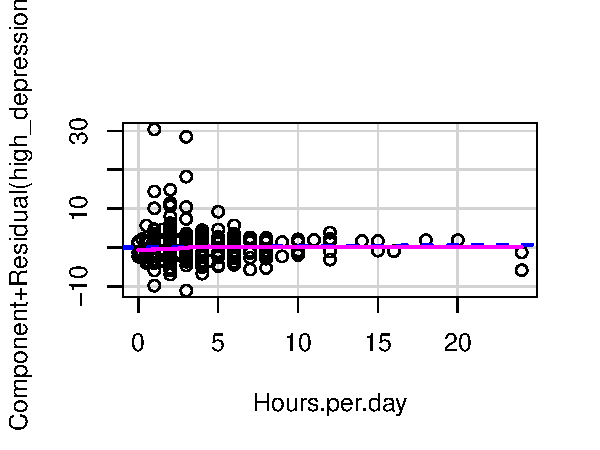
\includegraphics[keepaspectratio]{final_report_files/figure-pdf/unnamed-chunk-4-1.pdf}}

Because logistic regression assumes that continuous predictors have a
linear relationship with the log--odds of the outcome, we began by
checking this assumption for Hours per day using a
component--plus--residual (partial residual) plot. This plot did not
reveal strong curvature or systematic departures from linearity, as the
pink line was fitted very tightly to the blue, so we retained Hours per
day in linear form.

We then examined several additional diagnostics. First, we used VIFs to
assess multicollinearity among the predictors and did not detect
problematic levels of collinearity. Second, we evaluated overall model
fit with a Hosmer--Lemeshow goodness--of--fit test, which revealed a
p-value greater than 0.05 (0.1641), meaning the test indicates no
substantial issue with the fitting of the model.

We calculated leverage values using the hat matrix and identified
several observations above the common threshold of \(2\bar{h}\).
However, high leverage alone is not sufficient evidence to remove points
in logistic regression, particularly in models with many categorical
predictors. Because these cases did not show extreme Pearson residuals
either, we retained all observations for the final model.

\begin{longtable}[t]{rrrrrrrrrrrr}
\caption{Table 3: Confusion Matrix and Classification Metrics}\\
\toprule
TN & FP & FN & TP & Accuracy & Kappa & Sensitivity & Specificity & Precision & Recall & F1 & Balanced Accuracy\\
\midrule
277 & 95 & 103 & 243 & 0.724 & 0.447 & 0.719 & 0.729 & 0.702 & 0.719 & 0.711 & 0.724\\
\bottomrule
\end{longtable}

To assess predictive performance, we computed an initial confusion
matrix (Table 3) based on the conventional 0.5 probability threshold.
The initial confusion matrix showed 277 true negatives, 243 true
positives, 95 false negatives, and 103 false positives, yielding an
overall accuracy of 0.724. Sensitivity was 0.719, meaning the model
correctly identified about 72\% of participants with high depression,
while specificity was 0.729, indicating a similar rate of correct
classification among low-depression participants. The model's precision
(0.702) and F1 score (0.711) suggested moderate predictive performance
but also revealed room for improvement, particularly in reducing false
negatives.

\pandocbounded{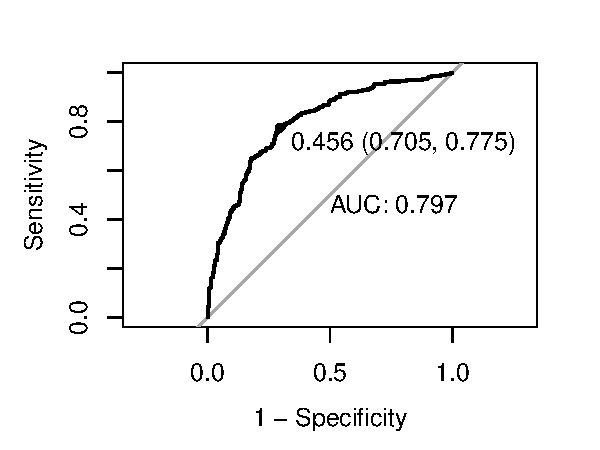
\includegraphics[keepaspectratio]{final_report_files/figure-pdf/unnamed-chunk-6-1.pdf}}

To further assess model performance, we examined the ROC curve and
computed the AUC. The model achieved an AUC of 0.797, indicating strong
discriminative ability. The optimal classification threshold was
identified as 0.456, which balances sensitivity and specificity more
effectively than the default 0.50 cutoff.

\begin{longtable}[t]{rrrrrrrrrrrr}
\caption{Table 4: Confusion Matrix and Classification Metrics (Threshold = 0.456).}\\
\toprule
TN & FP & FN & TP & Accuracy & Kappa & Sensitivity & Specificity & Precision & Recall & F1 & Balanced Accuracy\\
\midrule
268 & 76 & 112 & 262 & 0.738 & 0.478 & 0.775 & 0.705 & 0.701 & 0.775 & 0.736 & 0.74\\
\bottomrule
\end{longtable}

At this optimized threshold, we recomputed the confusion matrix (Table
4), and sensitivity increased from 0.719 to 0.775, meaning the model
detected a larger proportion of high-depression cases, while specificity
remained reasonably high at 0.705. Overall accuracy also improved from
0.724 to 0.738, and the F1 score increased from 0.711 to 0.736,
demonstrating that threshold adjustment meaningfully enhanced the
model's ability to classify high depression symptoms.

Finally, we tested whether hours per day meaningfully improved the
logistic regression model by comparing the full model to a reduced model
that excluded this predictor. A likelihood ratio test showed no
significant improvement from adding hours per day
\((\chi^2(1) = 2.23,\; p = 0.135)\), indicating that daily
music-listening hours do not provide additional explanatory power for
predicting high depression symptoms once other factors are accounted
for. Model fit indices aligned with this result: the AIC values for the
reduced and full models were nearly identical (839.39 vs.~839.16),
confirming that including hours per day does not meaningfully enhance
model performance. However, because our research question specifically
examines the role of daily listening time, we retain the full model as
our primary specification.

\begin{longtable}[t]{lrrrlrr}
\caption{Table 5: Logistic regression model for RQ2 (odds ratios with 95 percent confidence intervals).}\\
\toprule
Term & Odds Ratio & Std Error & statistic & p-value & 2.5\% CI & 97.5\% CI\\
\midrule
(Intercept) & 0.08 & 0.52 & -4.8161509 & p<0.001 & 0.03 & 0.22\\
Hours.per.day & 1.05 & 0.03 & 1.4764301 & 0.140 & 0.99 & 1.12\\
Age & 0.99 & 0.01 & -1.4976696 & 0.134 & 0.97 & 1.00\\
InstrumentalistYes & 0.94 & 0.22 & -0.2893564 & 0.772 & 0.61 & 1.43\\
ComposerYes & 1.13 & 0.26 & 0.4570654 & 0.648 & 0.68 & 1.87\\
\addlinespace
Anxiety & 1.40 & 0.04 & 8.6830117 & p<0.001 & 1.30 & 1.51\\
Insomnia & 1.17 & 0.03 & 5.0936882 & p<0.001 & 1.10 & 1.24\\
OCD & 0.97 & 0.03 & -0.7990682 & 0.424 & 0.91 & 1.04\\
Fav.genreCountry & 0.57 & 0.59 & -0.9522194 & 0.341 & 0.17 & 1.79\\
Fav.genreEDM & 1.18 & 0.53 & 0.3036052 & 0.761 & 0.41 & 3.37\\
\addlinespace
Fav.genreFolk & 0.79 & 0.53 & -0.4380352 & 0.661 & 0.28 & 2.26\\
Fav.genreGospel & 0.20 & 1.30 & -1.2446057 & 0.213 & 0.01 & 1.99\\
Fav.genreHip hop & 2.54 & 0.54 & 1.7321500 & 0.083 & 0.90 & 7.49\\
Fav.genreJazz & 0.72 & 0.61 & -0.5339638 & 0.593 & 0.21 & 2.42\\
Fav.genreK pop & 0.41 & 0.61 & -1.4771463 & 0.140 & 0.12 & 1.32\\
\addlinespace
Fav.genreLatin & 1.01 & 1.58 & 0.0063683 & 0.995 & 0.03 & 32.42\\
Fav.genreLofi & 1.98 & 0.83 & 0.8259485 & 0.409 & 0.42 & 11.47\\
Fav.genreMetal & 1.17 & 0.42 & 0.3797032 & 0.704 & 0.51 & 2.70\\
Fav.genrePop & 0.66 & 0.41 & -1.0317028 & 0.302 & 0.30 & 1.46\\
Fav.genreR and B & 0.73 & 0.55 & -0.5711555 & 0.568 & 0.24 & 2.13\\
\addlinespace
Fav.genreRap & 0.63 & 0.62 & -0.7514045 & 0.452 & 0.18 & 2.09\\
Fav.genreRock & 1.30 & 0.38 & 0.6954891 & 0.487 & 0.62 & 2.77\\
Fav.genreVideo game music & 0.57 & 0.49 & -1.1384220 & 0.255 & 0.21 & 1.50\\
Music.effectsNo effect & 1.11 & 0.21 & 0.4851821 & 0.628 & 0.73 & 1.69\\
Music.effectsWorsen & 2.60 & 0.60 & 1.5973620 & 0.110 & 0.84 & 9.14\\
\bottomrule
\end{longtable}

Table 5 summarizes the corresponding regression results on the
odds--ratio scale, including odds ratios, standard errors, confidence
intervals, and p--values. Daily hours spent listening to music showed no
significant association with high depression (OR = 1.05, 95\% CI:
0.99--1.12, \(p = 0.140\)), indicating that each additional hour of
listening time does not meaningfully change the odds of reporting
elevated depression symptoms. Age was also non-significant (OR = 0.99,
95\% CI: 0.97--1.00, \(p = 0.134\)), suggesting that depression levels
did not vary systematically across ages in this sample.

The only strong and consistent predictors were mental--health variables
already closely tied to depression. Anxiety had a large, significant
effect (OR = 1.40, 95\% CI: 1.30--1.51, \(p < 0.001\)), meaning that
each one-unit increase in anxiety score increased the odds of high
depression by approximately 40\%. Insomnia also significantly increased
risk (OR = 1.17, 95\% CI: 1.10--1.24, \(p < 0.001\)). OCD symptoms were
not significant (OR = 0.97, \(p = 0.424\)).

Neither musician status (Instrumentalist or Composer) nor any
favorite--genre category significantly predicted high depression, as all
confidence intervals crossed 1.0. Although ``Music effects: worsen'\,'
had a relatively large odds ratio (OR = 2.60), the estimate was
imprecise (95\% CI: 0.84--9.14, \(p = 0.110\)) and therefore not
statistically reliable.

Overall, the model indicates that depression symptoms are most strongly
predicted by other co-occurring mental--health indicators (anxiety and
insomnia), whereas hours of music listening, demographic variables,
musician traits, and musical preferences show no meaningful association
with elevated depression levels.

\subsection{Limitations}\label{limitations}

Our analysis has several important limitations that should be kept in
mind when interpreting the results.

\begin{itemize}
\item
  \textbf{Self-reported and cross-sectional data:} All variables in the
  dataset, including mental-health symptoms and daily listening habits,
  were self-reported. This introduces potential measurement error due to
  inaccurate recall, inconsistent interpretation of questions, or social
  desirability bias. Additionally, because the data is cross-sectional,
  we cannot determine temporal ordering or causality. For instance, even
  if hours of listening were associated with depression, we cannot know
  whether listening more contributes to symptoms or whether individuals
  with higher depression simply listen to more music.
\item
  \textbf{Limited measurement of key variables:} Several important
  constructs were captured using single questions (for example, music
  effects, listening to music while working, and favorite genre), which
  restricts measurement precision. Some mental-health scores may also
  overlap conceptually, as illnesses like anxiety and insomnia strongly
  correlate with depression. This makes it difficult to isolate unique
  events even when multicollinearity diagnostics appear acceptable.
\item
  \textbf{Simplified representation of music behavior:} Daily hours of
  listening is an extremely limited measure of music engagement. It does
  not capture when people listen (morning vs.~late night), how they
  listen (active vs.~passive), why they listen (mood regulation,
  entertainment, background noise), or what they listen to within
  genres, all of which could meaningfully relate to mental-health
  outcomes. Similarly, ``primary streaming service'' does not capture
  multi-platform use or variability in content algorithms.
\item
  \textbf{Missing potential confounders:} Several important correlated
  variables of depression, like socioeconomic status, employment,
  physical health, sleep patterns, chronic stress, and academic
  workload, were not measured. Their absence means our model may suffer
  from omitted-variable bias, limiting the interpretability of estimated
  relationships.
\end{itemize}

\subsection{Future Work}\label{future-work}

To strengthen the results and analysis, several steps could be taken in
future research:

\begin{itemize}
\tightlist
\item
  \textbf{Collect richer and more detailed data:} Future studies would
  benefit from using validated multi-item psychological scales, such as
  PHQ-9 for depression or GAD-7 for anxiety, rather than the single
  self-reported questions on a scale of 0-10. Incorporating more
  granular measures of music engagement, such as listening context,
  emotional motivation, time-of-day patterns, or track-level
  characteristics, would also allow for more accurate modeling of how
  different aspects of music behavior relate to mental-health outcomes.
\item
  \textbf{Use longitudinal or experimental study designs:} Because the
  current dataset is cross-sectional, it cannot speak to temporal
  ordering or causal relationships. Longitudinal surveys could help
  determine whether music-listening habits change before shifts in mood
  or vice-versa. Experimental designs, such as one that involves
  assigning participants to specific listening conditions, would further
  clarify causal pathways.
\item
  \textbf{Apply more flexible modeling approaches:} Although linear and
  logistic regression provided interpretable results, more flexible
  models that are outside the scope of this class, like generalized
  additive models, random forests, or gradient-boosted trees, could
  capture non-linear relationships and interactions that traditional
  parametric models may miss. These models could also improve predictive
  accuracy, especially if supplemented with richer features.
\item
  \textbf{Address unmeasured confounders and broaden co-variates:}
  Adding variables related to sleep quality, stress, socioeconomic
  status, work or academic pressure, or physical health would reduce
  omitted-variable bias. These variables are often meaningful predictors
  of depression and may help clarify whether music-listening habits have
  independent effects.
\item
  \textbf{Expand the scope of musical data:} Streaming-platform logs or
  acoustic features from tracks (tempo, energy, valence, etc.) would
  enable more detailed analysis of how specific music properties or
  listening patterns relate to mental-health symptoms. This would move
  the analysis beyond total hours per day and allow for deeper
  behavioral insights.
\end{itemize}

These limitations mean that our findings should be interpreted as
descriptive patterns in this sample, rather than definitive evidence
about the causal effect of music listening on depression. Nonetheless,
the analysis provides a useful starting point for understanding how
music--listening habits and mental--health symptoms co--vary in this
population.




\end{document}
